\chapter{Simulator}
The simulator general objective is to have a instrument to validate our ideas and results in a experimental way. In particular we want obtain experimentally for each task, the distribution of job execution time.

%%%%%%%%%%%%%%%%%%%%%%%%%%%%%%%%%%%%%%%%%%%%%%%%%
\section{Taskset Model}
\label{sec:task_model}
In this section we define the taskset model, i.e., how the tasks in the taskset can be defined and which are their non functional characteristics.
From now on we suppose that:
\begin{itemize}
    \item We suppose to have a single core CPU.
    \item Each task is independent from the others. This means that there aren't shared resources among two tasks.
    \item Each task have a single elementary execution unit, i.e. each task have only one chunk.
    \item The task execution time is defined probabilistically, i.e. the execution time of each task is sampled from some distribution; this includes also the deterministic one.
    \item The jobs execution time are i.i.d. (i.e., independent and identically distributed). This means that only one distribution that represents the job execution time pattern of a given task. Maybe at the end we will move towards a model in which we can define a relation between job execution time.
    \item Task can be both periodic and sporadic (i.e. the releases between two consecutive job of the same task are separated from a minimum inter-arrival time). This releasing time is defined in a probabilistic way by some distribution.
\end{itemize}

%%%%%%%%%%%%%%%%%%%%%%%%%%%%%%%%%%%%%%%%%%%%%%%%%
\section{Input and Output}
The simulator input are the following:
\begin{itemize}
    \item A fixed priority scheduling algorithm.
    \item The taskset characterized from the assumptions in Section~\ref{sec:task_model}.
    \item The duration of the simulation.
\end{itemize}

\myskip

The outputs are the Cumulative Distribution Function (CDF) and the Probability Density Function (PDF) of the job execution time distribution for each task.

\myskip

To test the scheduler algorithm implementation, the simulator produces a file, named \textit{trace.log}, containing a sequence of \textit{<time, event>}, where  \textit{event} can be: the release of a job, the execution of a job, the completion of a job and the task preemption.

%%%%%%%%%%%%%%%%%%%%%%%%%%%%%%%%%%%%%%%%%%%%%%%%%
\section{Implementation}
In Figure~\ref{fig:class_diagram} is shown the class diagram of the simulator. The following elements are the core component of the simulator.

\begin{itemize}
    \item[\textbf{TaskSet}] Is a simple set of all task.
    \item[\textbf{Task}] The class \texttt{Task.java} represent a task. We can see it like the project, the static element modeling the task characteristic: period, deadline and the execution time; the first two are expressed by \texttt{Duration} objects, where the time must be expressed in milliseconds, while the last is a Sirio \texttt{Sampler}. It also maintains an internal \texttt{jobCounter} to uniquely identify its jobs.
    \item[\textbf{Job}] The class \texttt{Job.java} represent a task instance. While a Task contain only the task specifications, a Job contains the active state: its release time, its absolute deadline, the remaining execution time and the information about its completeness. It handle also the execution activity.
    \item[\textbf{Scheduler}] The class \texttt{Scheduler.java} represent the heart of the simulation. It handles the main structures: \textit{readyJobs}, a ready to execute job queue (i.e., a \texttt{TreeSet}) ordered by their priority; \textit{activeJobs}, maintain for each task the job that are actually in life, useful to identify a deadline miss; \textit{events}, a list with all interest instants for the simulation generated by the \texttt{Utils} class. It also manages \textit{blockedJobs} for future extensions.
    \item[\textbf{DMScheduler}] Is a specialization of the general Scheduler. It handles the priority assignment. For Deadline Monotonic the priority of a task is assigned in reverse ordering respect its deadline.
\end{itemize}

\begin{figure}[htbp]
    \centering
    
\includegraphics[max width=\textwidth, max height=0.85\textheight, keepaspectratio]{images/1-simulator/class diagram.pdf}
    \caption{Simulator Class Diagram.}
    \label{fig:class_diagram}
\end{figure}

\subsection{Utilities}
Let's observe the utilities used by more classes:
\begin{itemize}
    \item [\textbf{SampleDuration}] This class is useful to obtain a Duration object given a Sirio distribution. This duration represent time in nanoseconds as described in Section~\ref{subsec:simulator_time}.
    \item [\textbf{ConstantSampler}] A specialization of the Sirio \texttt{Sampler} interface that always returns a constant value, used for deterministic parameters like deadlines.
    \item [\textbf{TraceLogger}] An interface that abstracts the logging operations, implemented by \texttt{MyLogger}.
    \item [\textbf{MyLogger}] Is a helper class that abstracts the logging operation with a personalized format, writing to a file named \textit{trace.log}.
    \item [\textbf{MyClock}] Represents the global clock of the system. Implements the method to go at specified time, to go forward in time by a specified duration and to print the current time.
    \item [\textbf{Utils}] Provides static methods like \texttt{generatePeriodUpToMax} to calculate all relevant simulation events.
    \item [\textbf{DeadlineMissedException}] A custom exception thrown when a task exceeds its deadline, interrupting the simulation.
\end{itemize}

\subsection{Flow}
Let's analyse, thanks also to the Figure~\ref{fig:activity_diagram},the scheduler flow. This follow the steps below:
\begin{enumerate}
    \item Reset the state of the whole system. This allow the client to call more and more time \texttt{analyze()}.
    \item Release the first job of all tasks.
    \item Calculate the relevant events: these are all the multiples of tasks periods up to the simulation duration.
    \item Iterate through all events.
    \begin{enumerate}
        \item Calculate the available time from now to the next event.
        \item Distribute the available time among all ready jobs according to their priority.
        \item Advance to the next event.
        \item Release those tasks whose period matches the current time. The release of the new job is the moment when it sampling its execution time.
    \end{enumerate}
\end{enumerate}

\begin{figure}[htbp]
    \centering
    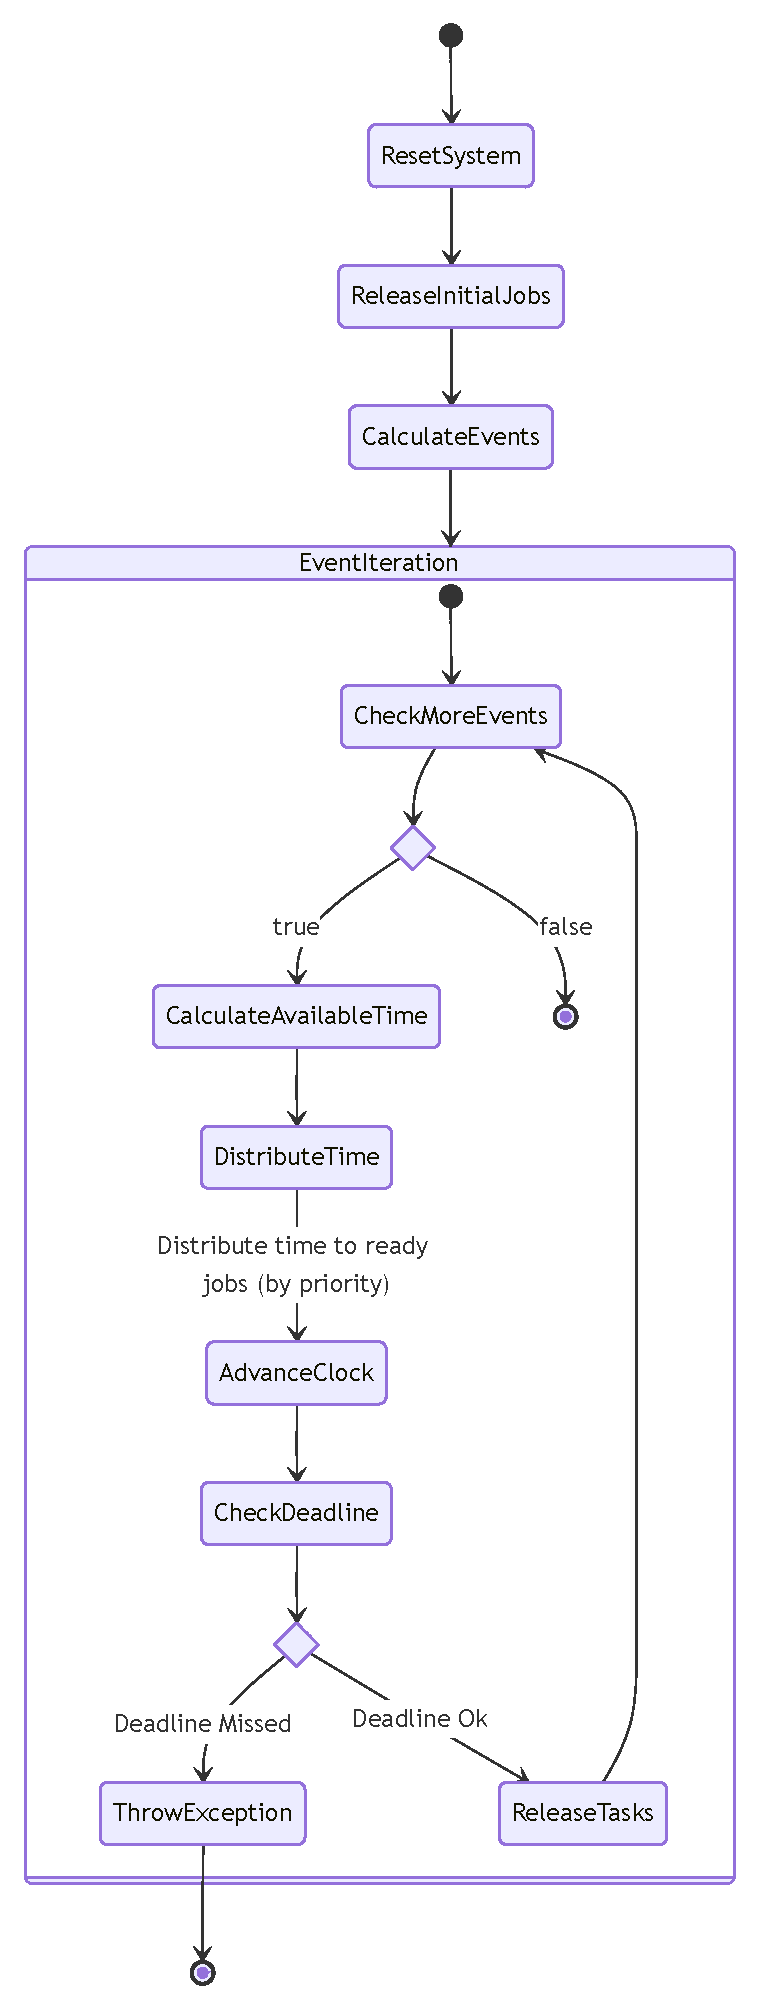
\includegraphics[max width=\textwidth, max height=0.85\textheight, keepaspectratio]{images/1-simulator/activity_diagram.pdf}
    \caption{Simulator Activity Diagram.}
    \label{fig:activity_diagram}
\end{figure}

\subsection{Time}
\label{subsec:simulator_time}
This kind of simulation must be totally deterministic; for this reason all timing aspects have been handle in a discrete way using the \texttt{Duration} Java type. In this way we can handle the complexity of small duration with a high abstraction level.

We assume that the time is taken in input and returned in output in millisecond. During the execution, to obtain the maximum precision, it is elaborated in nanoseconds.

\myskip

Related to timing, the system has obviusually the capabilities to identifies a deadline miss by a task and can also identifies the job that is responsable of this violation. This check is implemented by a single function (i.e., we have a single poit of truth) called after each time advancement: this allow us to identifies both the violation during the job execution and during the its subspention.

A violation implies the abort of whole simulation.